\begin{frame}{stateful firewall}
    \begin{itemize}
    \item common policy: allow outgoing connections only
    \vspace{.5cm}
    \item prior approach:
        \begin{itemize}
        \item drop incoming non-TCP, or TCP SYN
        \end{itemize}
    \item problems:
        \begin{itemize}
        \item disallowing UDP-based protocols (example: DNS over UDP, HTTP/3)
        \item disallowing normal ICMP (example: ICMP ping replies)
        \item allowing unsolicited TCP packets
        \end{itemize}
    \end{itemize}
\end{frame}

\begin{frame}{keeping state}
    \begin{itemize}
    \item outgoing connections only?
    \item really want to track list of \textit{connections}
    \vspace{.5cm}
    \item most common form of \textit{stateful firewall}
    \end{itemize}
\end{frame}

\begin{frame}{connection tracking?}
    \begin{itemize}
    \item simple idea for TCP:
    \item see SYN: add (TCP, source IP+port, dest IP+port) to table
    \item see FIN, FIN+ACK, ACK: remove row from table after timeout
    \item (plus other timeouts, error cases, etc.)
    \vspace{.5cm}
    \item mirrors TCP state machine
    \end{itemize}
\end{frame}

\begin{frame}{Linux conntrack}
    \begin{itemize}
    \item in-kernel table of active ``connections''
    \item includes notion of connections for UDP, ICMP, etc.
        \begin{itemize}
        \item heuristic guesses since protocol has no connect/close operation
        \end{itemize}
    \item maintains table of (proto, source host+port, dest host+port)
    \item packets marked with connection state
        \begin{itemize}
        \item new, established, \myemph<2>{related}, invalid
        \end{itemize}
    \end{itemize}
\end{frame}

\begin{frame}{related connection example}
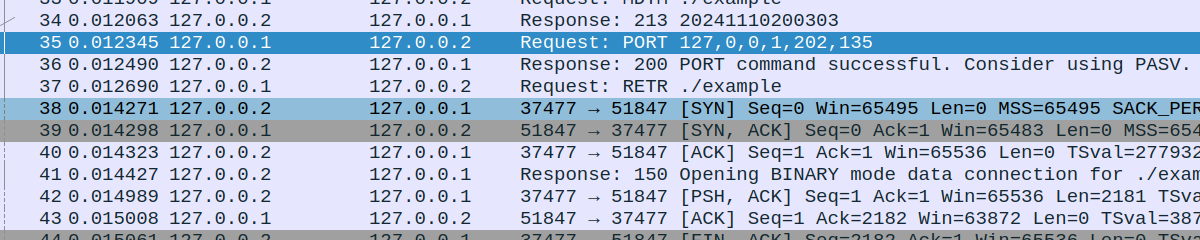
\includegraphics[width=\textwidth]{../fire/ftp-port-ex.png}
\begin{itemize}
\item FTP --- uses separate control + data TCP connections
\vspace{.5cm}
\item PORT command: server creates data connection to specified address
    \begin{itemize}
    \item $202 \times 256 + 135 = 51847$
    \item problem for firewalls: looks like `fresh' TCP connection
    \end{itemize}
\end{itemize}
\end{frame}

\begin{frame}{FTP: server connect to client?}
\begin{itemize}
\item PORT command: server creates data connection to specified address
\item PASV command: server gets address for client to conect
    \begin{itemize}
    \item most FTP clients default to this mode
    \end{itemize}
\item why both: in theory, allows direct server-to-server transfers
    \begin{itemize}
    \item one client uses PASV on one server, PORT on the other
    \end{itemize}
\end{itemize}
\end{frame}

\begin{frame}{other related connections Linux supports}
    \begin{itemize}
    \item usually: separate control and data connections
        \begin{itemize}
        \item esp. when data sent with UDP or from different machine
        \end{itemize}
    \vspace{.5cm}
    \item direct-client-to-client file transfers in Internet Relay Chat
    \item SIP, H.323 (video/audio call/conferencing protocols)
    \item PPTP (VPN protocol)
    \end{itemize}
\end{frame}

\begin{frame}[fragile]{nft with conntrack}
\begin{Verbatim}
table inet filter {
    chain input {
        type filter hook input priority 0

        ct state established accept
        ct state related accept
        ct state invalid drop
        iifname ethInt ct state new accept
        drop
    }
}
\end{Verbatim}
\end{frame}

\begin{frame}{connection state timeouts}
    \begin{itemize}
    \item problem: TCP connection with no activity for 30 minutes
    \item should it stay in table?
    \item how about after 8 hours?
    \vspace{.5cm}
    \item Linux conntrack, configurable timeouts:
        \begin{itemize}
        \item default: 5 days if in ESTABLISHED TCP state machine state
        \item lower for other connection TCP states (e.g. middle of handshake)
        \end{itemize}
    \item could disagree with end-host timeouts!
        \begin{itemize}
        \item mysterious connection dropping
        \end{itemize}
    \end{itemize}
\end{frame}

\begin{frame}{TCP keep-alive}
    \begin{itemize}
    \item for TCP: SO\_KEEPALIVE socket option
    \item enables periodic ``keep-alive'' messages
        \begin{itemize}
        \item periodically send empty probe packets, resend last byte of data
        \item threshold for number of probes after which to consider connection lost
        \end{itemize}
    \vspace{.5cm}
    \item also many protocols have periodic `ping/pong' messages
    \end{itemize}
\end{frame}
